\begin{figure}[t]
\centering
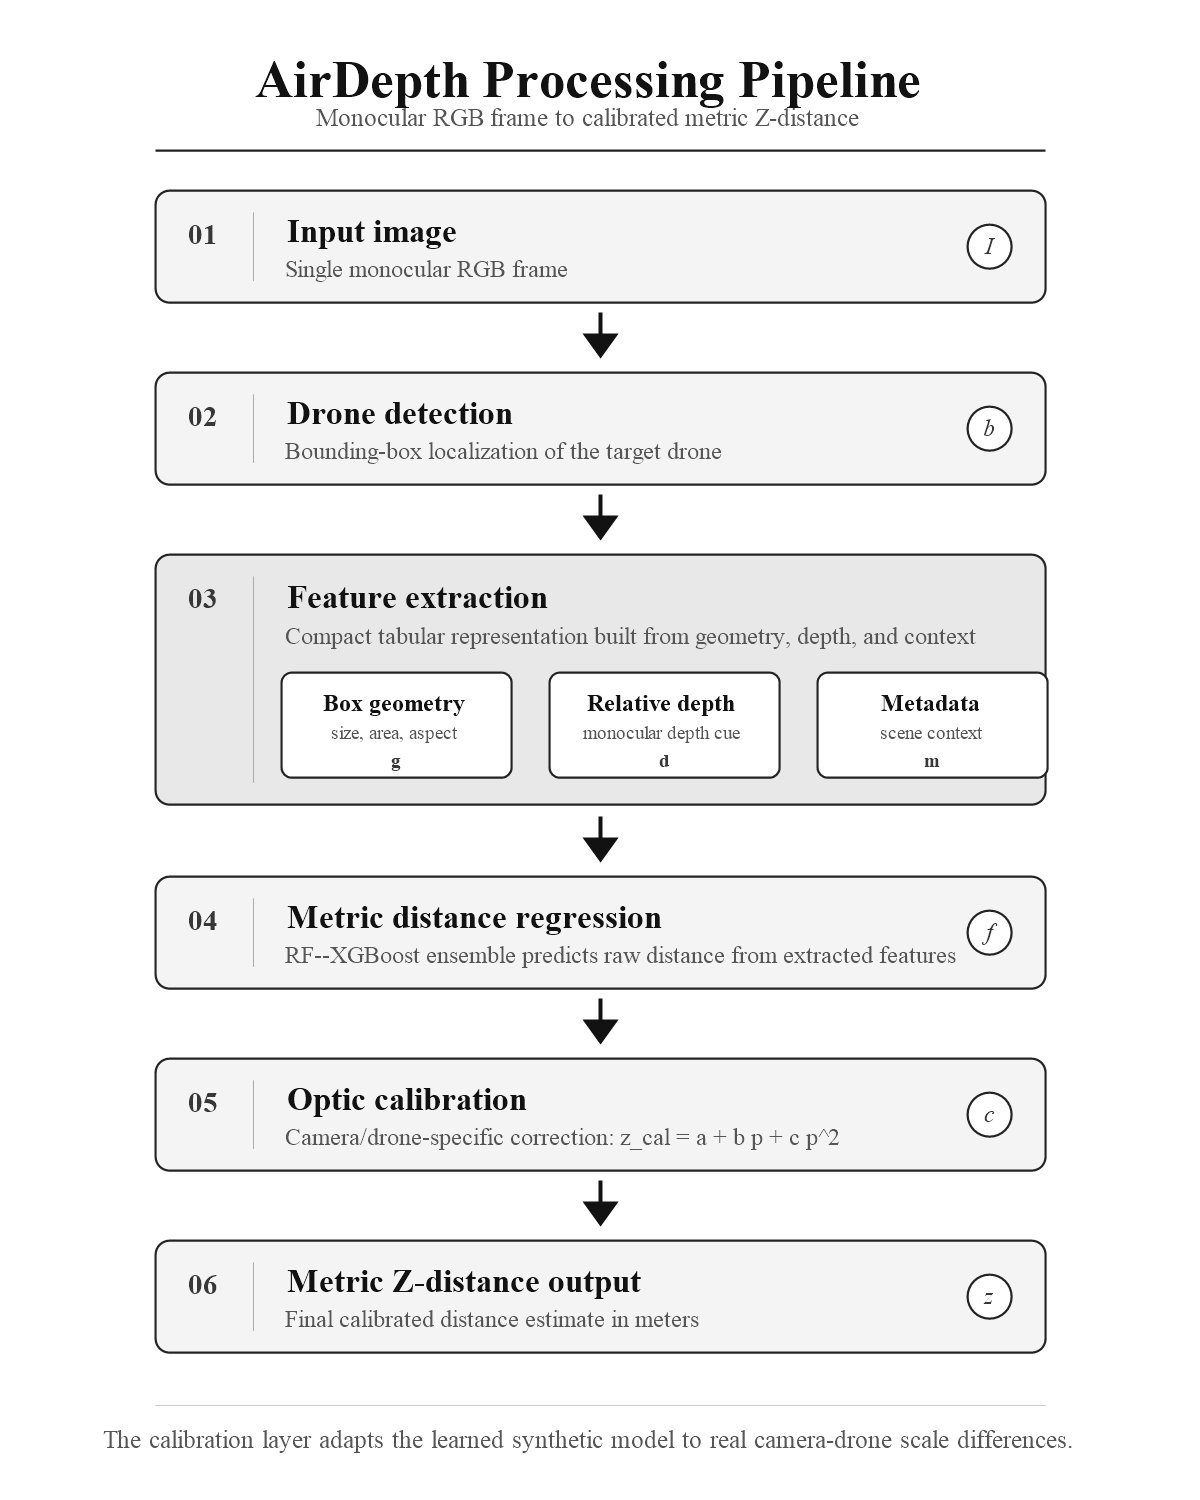
\includegraphics[width=\columnwidth]{Sections/Images/Pipeline.png}
\caption{AirDepth processing pipeline. A monocular RGB frame is first passed through drone detection, followed by feature extraction from bounding-box geometry, relative depth, and scene metadata. The extracted representation is processed by the RF--XGBoost distance regressor and then corrected by an optic calibration stage to produce the final metric Z-distance estimate.}
\label{fig:airdepth_pipeline}
\end{figure}
